\section{Resultados experimentales}
Se realizaron 3 experimentos para comprobar el funcionamiento del perceptrón multicapa, para cada experimento se introdujeron valores diferentes para cada parámetro de la arquitectura, esto debido a que cada función a aproximar necesita parámetros personalizados para su correcto funcionamiento.

Algunas constantes que se mantienen en todos los experimentos son que la entrada de datos y objetivos se realizan mediante archivos de texto, además para cada experimento se muestra la evolución del error de iteración de entrenamiento y de validación en estas gráficas se puede observar que el error de validación tiende a ser más alto que el error de entrenamiento.

También, se gráfica la evolución de pesos y bias para cada capa de la red neuronal, finalmente se muestra una comparación entre un conjunto de prueba y la salida que proporciona el MLP. Además de imprimir los valores finales de error de iteración, error de validación y error de prueba. Finalmente los valores finales de pesos y bias son almacenados en un archivo de texto, uno por cada capa de la red.
\subsection{Experimento 1}
Se trabajo con un conjunto de datos con 101 datos los cuales al graficar dan como resultado la figura \ref{fig:original1}.

Los valores que se ingresaron son los que se muestran en la figura \ref{fig:entrada1} los valores más importantes que se tienen aquí son el factor de aprendizaje $\alpha=0.03$ el máximo numero de iteraciones a realizar el cual fue $iteraciones_{max} = 5000$ junto a un error permitido de $E_{it} = 0.005$ mientras que cada $200$ iteraciones se hará una iteración de validación con un máximo de tres incrementos consecutivos.
\begin{figure}[H]
    \begin{center}
        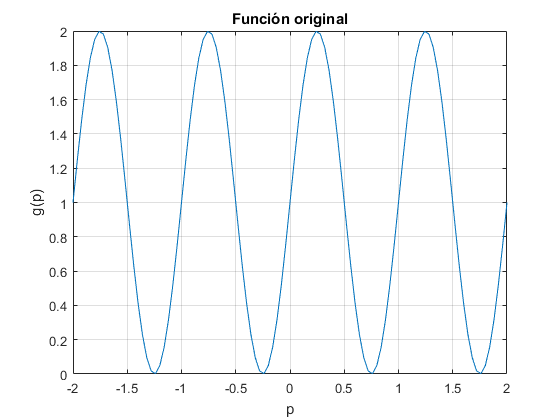
\includegraphics[width=10cm]{1/original.png}
        \caption{Función a aproximar en el experimento 1.}
        \label{fig:original1}
    \end{center}
\end{figure}
Para realizar las iteraciones de entrenamiento, prueba y validación la división del conjunto de datos fue $80-10-10$ respectivamente. Por otro lado, la arquitectura fue la siguiente.
\[ \left[ 1 \quad 6 \quad 1 \right] \]
\[ \left[ 3 \quad 1 \right] \]
donde
\begin{itemize}
    \item $3$ hace referencia a la función $tansig$.
    \item $1$ es la función $purelin$.
\end{itemize}
Una representación gráfica de esta arquitectura es la que se muestra en la figura \ref{fig:arqui1}. Los valores de pesos y bias de cada capa son inicializados entre $-1$ y $1$.
\begin{figure}[H]
    \begin{center}
        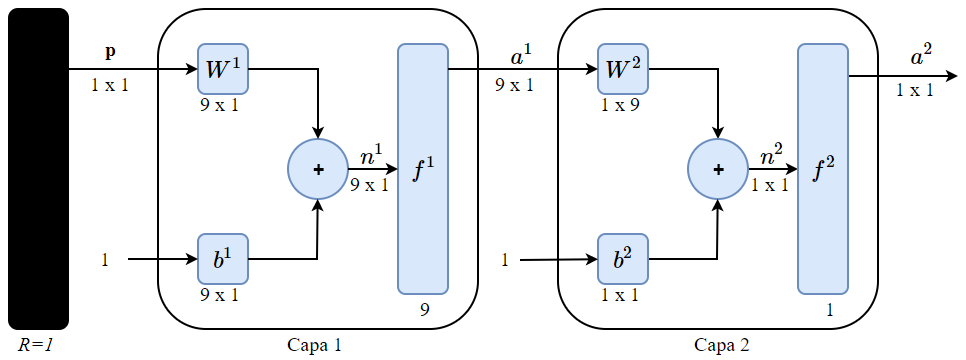
\includegraphics[width=14cm]{img/arqui1.png}
        \caption{Arquitectura del primer experimento.}
        \label{fig:arqui1}
    \end{center}
\end{figure}
Como se puede observar la primera capa tiene seis neuronas mientras que la segunda sólo tiene 1. Además las ecuaciones para la propagación hacia adelante y backpropagation se convierten en las siguientes.
\begin{figure}[H]
    \begin{align*}
        \boldsymbol{a}^0 &= \boldsymbol{p} \\
        \boldsymbol{a}^{1} &= logsig(\boldsymbol{W}^{1}\boldsymbol{a}^{0}+\boldsymbol{b}^{1}
        ) \\
        \boldsymbol{a}^{2} &= purelin(\boldsymbol{W}^{2}\boldsymbol{a}^{1}+\boldsymbol{b}^{2}
        ) \\
        \boldsymbol{a} &= \boldsymbol{a}^{2}
    \end{align*}
    \caption{Ecuaciones de propagación hacia adelante.}
\end{figure}
\begin{figure}[H]
    \begin{center}
        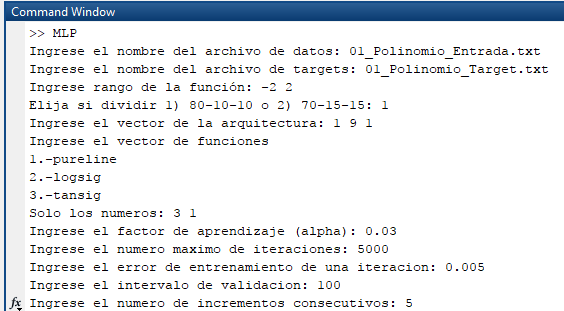
\includegraphics[width=14cm]{1/entrada.png}
        \caption{Entrada de datos del experimento 1.}
        \label{fig:entrada1}
    \end{center}
\end{figure}

\begin{figure}[H]
    \begin{align*}
    \boldsymbol{W}^{1}(k+1) &= \boldsymbol{W}^{1}(k) - \alpha \boldsymbol{s}^{1} (\boldsymbol{a}^{0})^T \\
    \boldsymbol{b}^{1}(k+1) &= \boldsymbol{b}^{1}(k) - \alpha \boldsymbol{s}^{1} \\
    \boldsymbol{W}^{2}(k+1) &= \boldsymbol{W}^{2}(k) - \alpha \boldsymbol{s}^{2} (\boldsymbol{a}^{1})^T \\
    \boldsymbol{b}^{2}(k+1) &= \boldsymbol{b}^{2}(k) - \alpha \boldsymbol{s}^{2} \\
    \boldsymbol{s}^2 &= 
    -2 \left[ 1 \right] (\boldsymbol{t-a}) \\
    \boldsymbol{s}^{1} &= 
    \boldsymbol{\dot{F}}^{1}(\boldsymbol{n}^{1})(\boldsymbol{W}^{2})^{T}
    \boldsymbol{s}^{2} \\
    \text{donde:} \\
    \boldsymbol{\dot{F}}^{1}(\boldsymbol{n}^{1}) &=
    \begin{bmatrix}
        1-(a_{1}^1)^2 & 0 & 0 & 0 & 0 & 0 \\
        0 & 1-(a_{2}^1)^2 & 0 & 0 & 0 & 0 \\
        0 & 0 & 1-(a_{3}^1)^2 & 0 & 0 & 0 \\
        0 & 0 & 0 & 1-(a_{4}^1)^2 & 0 & 0 \\
        0 & 0 & 0 & 0 & 1-(a_{5}^1)^2 & 0 \\
        0 & 0 & 0 & 0 & 0 & 1-(a_{6}^1)^2 \\
    \end{bmatrix}
    \end{align*}
    \caption{Ecuaciones del aprendizaje de la arquitectura de la figura \ref{fig:arqui1}.}
\end{figure}

\begin{figure}[H]
    \begin{center}
        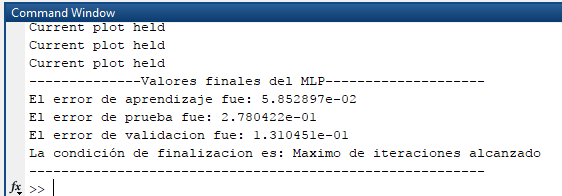
\includegraphics[width=14cm]{1/salida.png}
        \caption{Errores de cada iteración del experimento 1.}
        \label{fig:salida1}
    \end{center}
\end{figure}
Los errores finales se pueden observar en la figura \ref{fig:salida1}, además de que la condición de finalización fue que se alcanzo el número máximo de iteraciones.

Las siguientes imágenes son la evolución de pesos y bias de cada capa. Cada gráfica tiene comportamientos diferentes pero algo en lo que se parecen es que en algún punto de la gráfica ya no se producen tantas modificaciones en los valores que presentan.
\begin{figure}[H]
    \begin{center}
        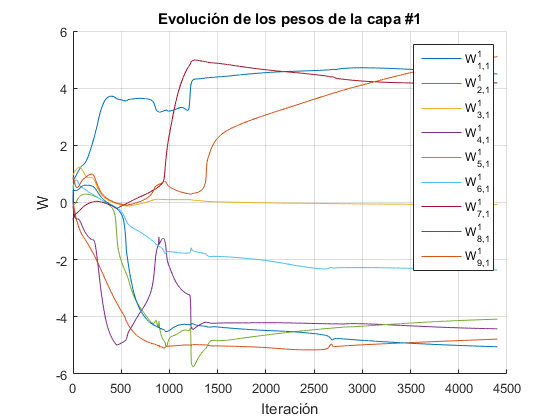
\includegraphics[width=12cm]{1/pesos1.png}
        \caption{Evolución de los pesos de la capa 1 del experimento 1.}
        \label{fig:pesos1}
    \end{center}
\end{figure}

\begin{figure}[H]
    \begin{center}
        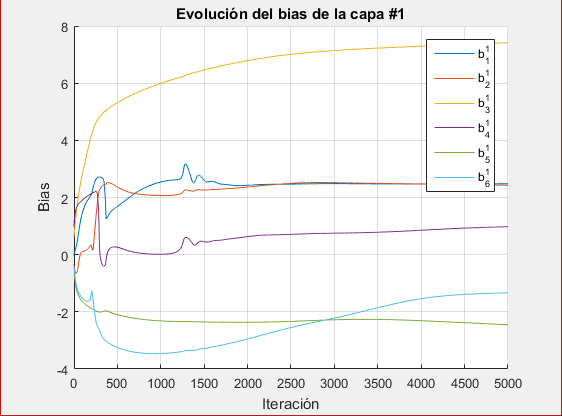
\includegraphics[width=12cm]{1/bias1.png}
        \caption{Evolución de los bias de la capa 1 del experimento 1.}
        \label{fig:bias1}
    \end{center}
\end{figure}

\begin{figure}[H]
    \begin{center}
        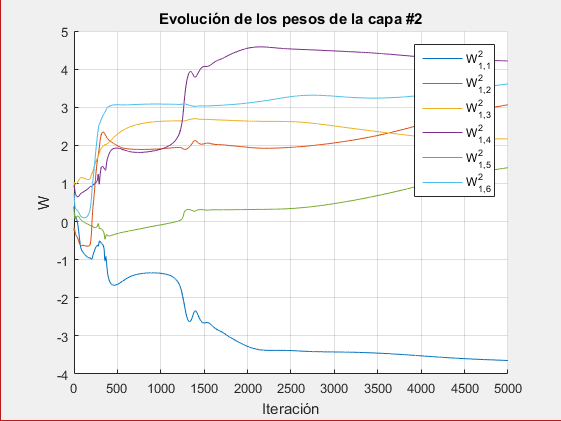
\includegraphics[width=12cm]{1/pesos2.png}
        \caption{Evolución de los pesos de la capa 2.}
        \label{fig:pesos2}
    \end{center}
\end{figure}

\begin{figure}[H]
    \begin{center}
        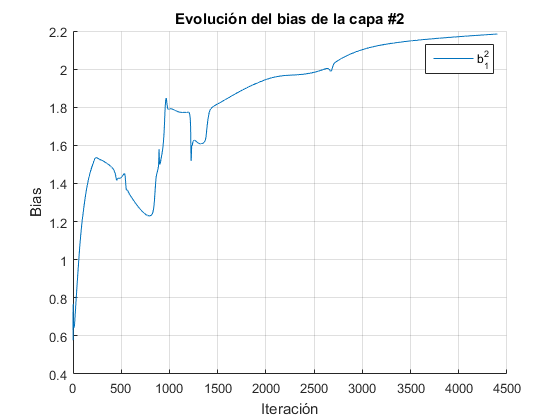
\includegraphics[width=12cm]{1/bias2.png}
        \caption{Evolución de los bias de la capa 2.}
        \label{fig:bias2}
    \end{center}
\end{figure}
Debido a que la división de los datos de entrada fue $80-10-10$ sólo se tienen $10$ datos que propagar se producen demasiados picos, por otro lado la aproximación se realiza casi completamente.
\begin{figure}[H]
    \begin{center}
        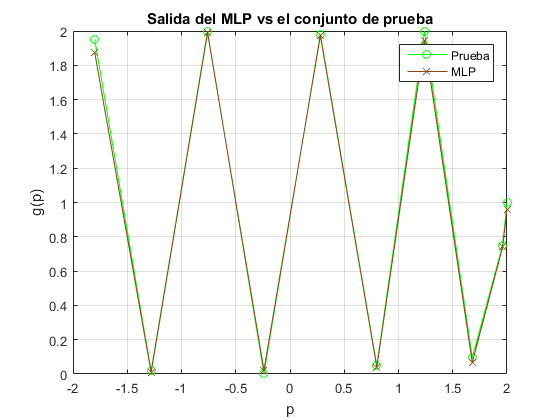
\includegraphics[width=12cm]{1/prueba.png}
        \caption{Comparación de las gráficas}
        \label{fig:prueba1}
    \end{center}
\end{figure}
Se puede observar que el error llega un punto en el que disminuye de una manera muy lenta hasta el final de todas las iteraciones.
\begin{figure}[H]
    \begin{center}
        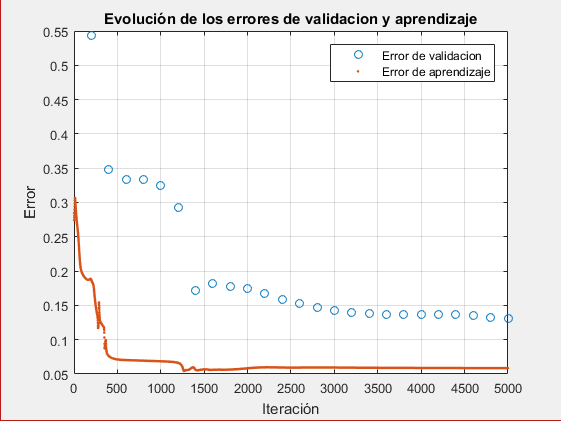
\includegraphics[width=16cm]{1/error.png}
        \caption{Evolución de los errores del experimento 1.}
        \label{fig:error1}
    \end{center}
\end{figure}
\newpage

\subsection{Experimento 2}
Para este experimento se trato con 241 datos los cuales al graficar dan como resultado la figura \ref{fig:original2}.

Los valores que se ingresaron son los que se muestran en la figura \ref{fig:entrada2} los valores más importantes que se tienen aquí son el factor de aprendizaje $\alpha=0.01$ el máximo numero de iteraciones a realizar el cual fue $iteraciones_{max} = 5000$ junto a un error permitido de $E_{it} = 0.0005$ mientras que cada $100$ iteraciones se hará una iteración de validación con un máximo de tres incrementos consecutivos.
\begin{figure}[H]
    \begin{center}
        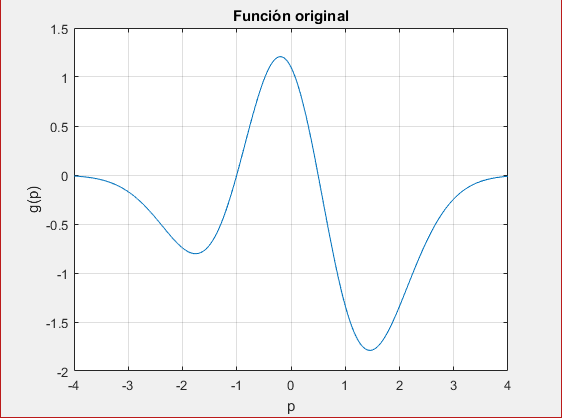
\includegraphics[width=12cm]{2/original.png}
        \caption{Función a aproximar en el experimento 2.}
        \label{fig:original2}
    \end{center}
\end{figure}
En esta ocasión la división de los datos fue $70-15-15$ para conjunto de entrenamiento, prueba y validación respectivamente. Por otro lado, la arquitectura fue la siguiente.
\[ \left[ 1 \quad 6 \quad 1 \right] \]
\[ \left[ 2 \quad 1 \right] \]
donde
\begin{itemize}
    \item $3$ hace referencia a la función $logsig$.
    \item $1$ es la función $purelin$.
\end{itemize}
Una representación gráfica de esta arquitectura es la que se muestra en la figura \ref{fig:arqui2}. Los valores de pesos y bias de cada capa son inicializados entre $-1$ y $1$.
\begin{figure}[H]
    \begin{center}
        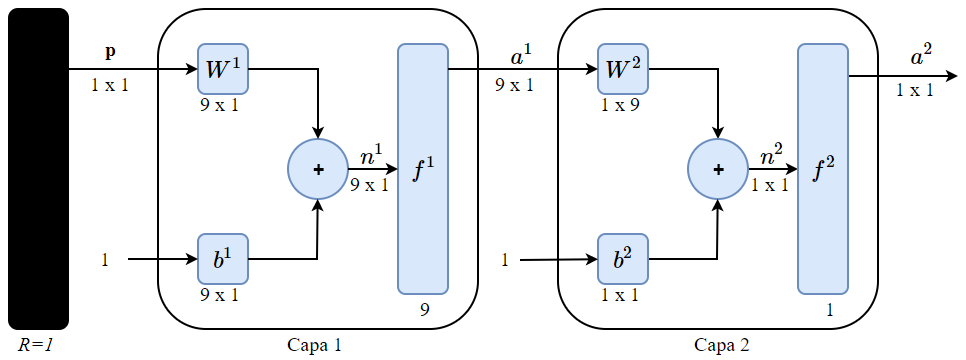
\includegraphics[width=14cm]{img/arqui1.png}
        \caption{Arquitectura del segundo experimento.}
        \label{fig:arqui2}
    \end{center}
\end{figure}
De nueva cuenta se tienen seis neuronas en la primera capa y sólo una en la segunda, lo cual genero las siguientes ecuaciones de propagación hacia adelante y backpropagation.

\begin{figure}[H]
    \begin{align*}
    \boldsymbol{a}^0 &= \boldsymbol{p} \\
    \boldsymbol{a}^{1} &= logsig(\boldsymbol{W}^{1}\boldsymbol{a}^{0}+\boldsymbol{b}^{1}
    ) \\
    \boldsymbol{a}^{2} &= purelin(\boldsymbol{W}^{2}\boldsymbol{a}^{1}+\boldsymbol{b}^{2}
    ) \\
    \boldsymbol{a} &= \boldsymbol{a}^{2}
    \end{align*}
    \caption{Ecuaciones de propagación hacia adelante.}
\end{figure}

\begin{figure}[H]
    \begin{center}
        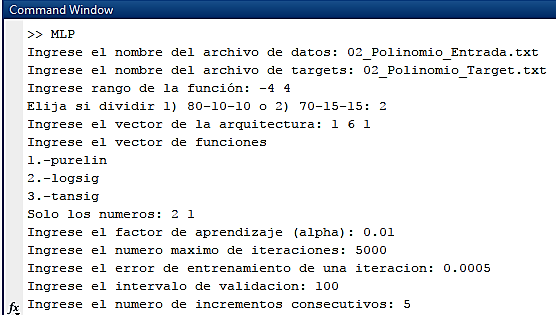
\includegraphics[width=14cm]{2/entrada.png}
        \caption{Entrada de datos del experimento 2.}
        \label{fig:entrada2}
    \end{center}
\end{figure}

\begin{figure}[H]
    \begin{align*}
    \boldsymbol{W}^{1}(k+1) &= \boldsymbol{W}^{1}(k) - \alpha \boldsymbol{s}^{1} (\boldsymbol{a}^{0})^T \\
    \boldsymbol{b}^{1}(k+1) &= \boldsymbol{b}^{1}(k) - \alpha \boldsymbol{s}^{1} \\
    \boldsymbol{W}^{2}(k+1) &= \boldsymbol{W}^{2}(k) - \alpha \boldsymbol{s}^{2} (\boldsymbol{a}^{1})^T \\
    \boldsymbol{b}^{2}(k+1) &= \boldsymbol{b}^{2}(k) - \alpha \boldsymbol{s}^{2} \\
    \boldsymbol{s}^2 &= 
    -2 \left[ 1 \right] (\boldsymbol{t-a}) \\
    \boldsymbol{s}^{1} &= 
    \boldsymbol{\dot{F}}^{1}(\boldsymbol{n}^{1})(\boldsymbol{W}^{2})^{T}
    \boldsymbol{s}^{2} \\
    \text{donde:} \\
    \boldsymbol{\dot{F}}^{1}(\boldsymbol{n}^{1}) &=
    \begin{bmatrix}
    (1-a_{1}^1)(a_{1}^1) & 0 & 0 & 0 & 0 & 0 \\
    0 & (1-a_{2}^1)(a_{2}^1) & 0 & 0 & 0 & 0 \\
    0 & 0 & (1-a_{3}^1)(a_{3}^1) & 0 & 0 & 0 \\
    0 & 0 & 0 & (1-a_{4}^1)(a_{4}^1) & 0 & 0 \\
    0 & 0 & 0 & 0 & (1-a_{5}^1)(a_{5}^1) & 0 \\
    0 & 0 & 0 & 0 & 0 & (1-a_{6}^1)(a_{6}^1) \\
    \end{bmatrix}
    \end{align*}
    \caption{Ecuaciones del aprendizaje de la arquitectura de la figura \ref{fig:arqui2}.}
\end{figure}

Los errores finales fueron, para el error de validación fue $2.61 x 10^{-3}$, para el de prueba fue $2.37x10^{-3}$ mientras que para el de aprendizaje fue $4.49x10^{-4}$ dichos valores se encuentran en la figura \ref{fig:salida2}, además de que la condición de finalización fue que el error de aprendizaje fue menor que el error de iteración.
\begin{figure}[H]
    \begin{center}
        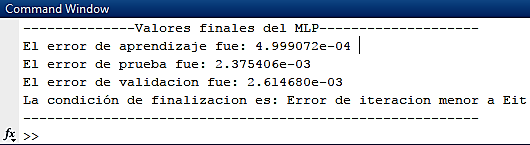
\includegraphics[width=14cm]{2/salida.png}
        \caption{Errores de cada iteración del experimento 2.}
        \label{fig:salida2}
    \end{center}
\end{figure}
Las siguientes imágenes son la evolución de pesos y bias de cada capa. Cada gráfica tiene comportamientos diferentes pero algo en lo que se parecen es que en algún punto de la gráfica ya no se producen tantas modificaciones en los valores que presentan.
\begin{figure}[H]
    \begin{center}
        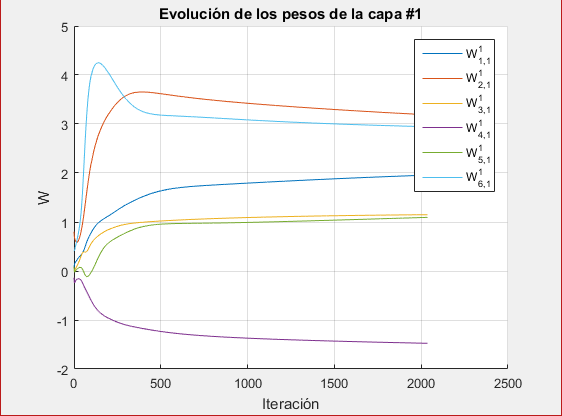
\includegraphics[width=13cm]{2/pesos1.png}
        \caption{Evolución de los pesos de la capa 1 del experimento 2.}
        \label{fig:pesos3}
    \end{center}
\end{figure}

\begin{figure}[H]
    \begin{center}
        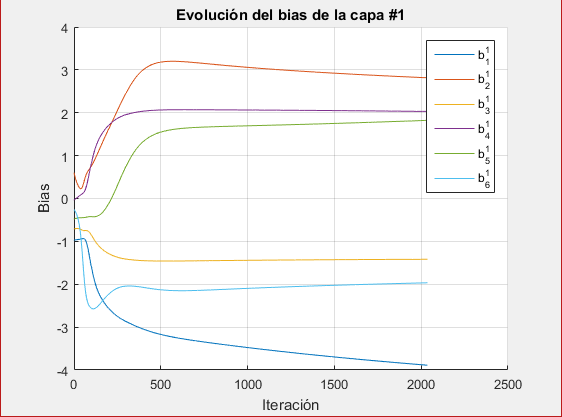
\includegraphics[width=13cm]{2/bias1.png}
        \caption{Evolución de los bias de la capa 1 del experimento 2.}
        \label{fig:bias3}
    \end{center}
\end{figure}

\begin{figure}[H]
    \begin{center}
        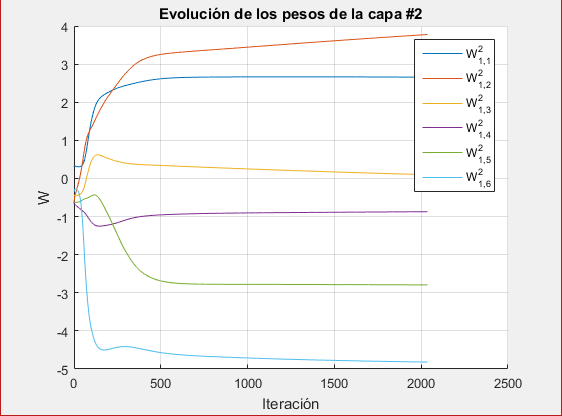
\includegraphics[width=13cm]{2/pesos2.png}
        \caption{Evolución de los pesos de la capa 2.}
        \label{fig:pesos4}
    \end{center}
\end{figure}

\begin{figure}[H]
    \begin{center}
        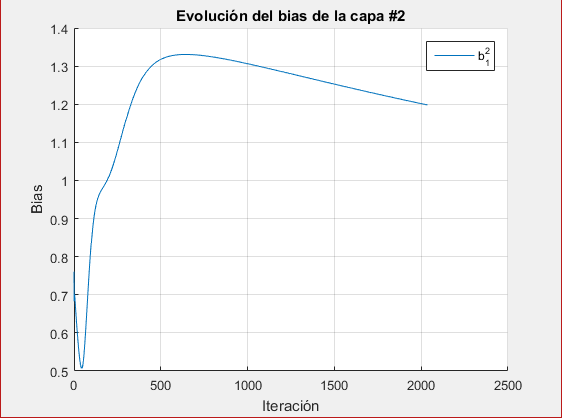
\includegraphics[width=13cm]{2/bias2.png}
        \caption{Evolución de los bias de la capa 2.}
        \label{fig:bias4}
    \end{center}
\end{figure}
Finalmente tenemos la comparación de la salida del MLP y los valores reales, ya que el error es muy bajo la aproximación se realiza en casi todos los puntos con excepción de los primeros valores de la gráfica
\begin{figure}[H]
    \begin{center}
        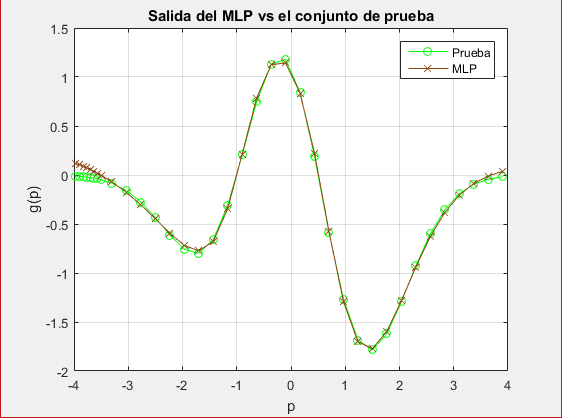
\includegraphics[width=16cm]{2/prueba.png}
        \caption{Comparación de las gráficas}
        \label{fig:prueba2}
    \end{center}
\end{figure}
El comportamiento de la gráfica anterior se puede ver reflejado en la evolución del error en el cual incluso el error de validación es más pequeño con cada iteración que se genera.
\begin{figure}[H]
    \begin{center}
        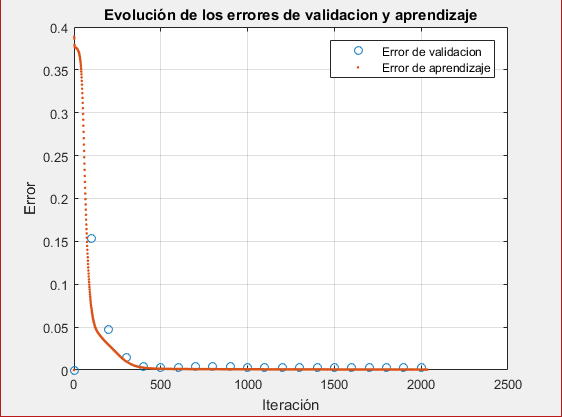
\includegraphics[width=16cm]{2/error.png}
        \caption{Evolución de los dos errores.}
        \label{fig:error2}
    \end{center}
\end{figure}

\newpage

\subsection{Experimento 3}
La cantidad de datos con los que se trabajo para este tercer experimento fueron 701 los cuales dan como resultado la gráfica que se muestra en la imagen \ref{fig:original3}.

Por otro lado, los parámetros que se utilizaron se encuentras en la figura \ref{fig:entrada3} es importante señalar los valores que juegan el papel más crucial en el funcionamiento del MLP los cuales son el factor de aprendizaje que fue$\alpha=0.005$, el máximo numero de iteraciones a realizar el cual fue $iteraciones_{max} = 5000$ y se tiene un error de iteración de $E_{it} = 0.0005$ además de tener este parámetro de finalización se debe realizar una iteración de validación cada $100$ iteraciones y si se detecta un incremento consecutivo tres veces se detendrá el aprendizaje para evitar el sobreentrenamiento.
\begin{figure}[H]
    \begin{center}
        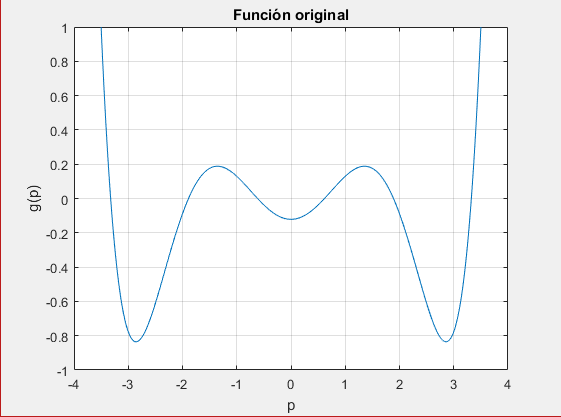
\includegraphics[width=14cm]{3/original.png}
        \caption{Función a aproximar en el experimento 3.}
        \label{fig:original3}
    \end{center}
\end{figure}
En esta ocasión la división de los datos fue $80-10-10$ para conjunto de entrenamiento, prueba y validación respectivamente. Por otro lado, la arquitectura fue la siguiente.
\[ \left[ 1 \quad 5 \quad 5 \quad 1 \right] \]
\[ \left[ 2 \quad 3 \quad 1 \right] \]
donde
\begin{itemize}
    \item $2$ hace referencia a la función $logsig$.
    \item $3$ hace referencia a la función $logsig$.
    \item $1$ es la función $purelin$.
\end{itemize}
Para que esta arquitectura sea más fácil de entender se presenta una representación gráfica de dicha arquitectura (véase figura \ref{fig:arqui3}). Al igual que en los experimentos anteriores los valores de pesos y bias son inicializados entre $-1$ y $1$.
\begin{figure}[H]
    \begin{center}
        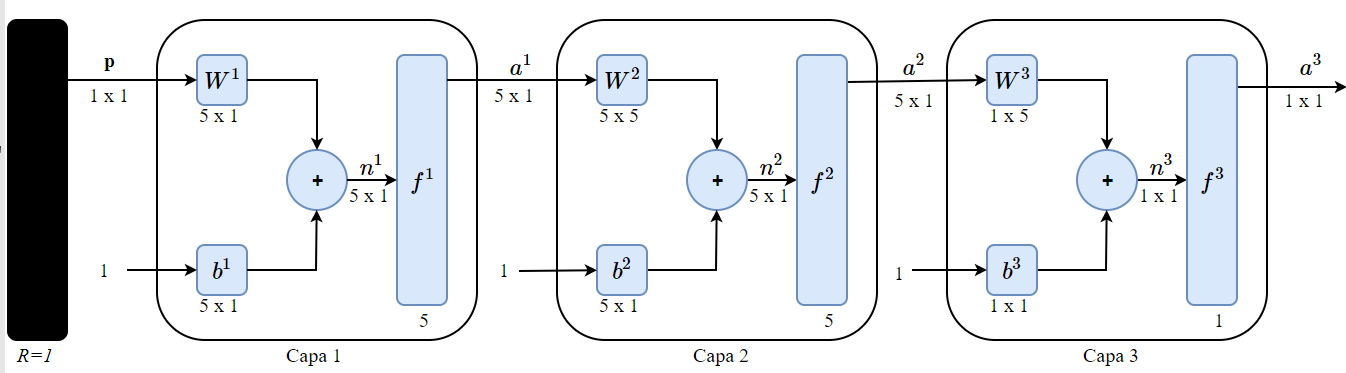
\includegraphics[width=16cm]{img/arqui3.png}
        \caption{Arquitectura del tercer experimento.}
        \label{fig:arqui3}
    \end{center}
\end{figure}
Como se puede observar, en este experimento no se tiene la misma arquitectura que en los experimentos anteriores ya que después de muchas pruebas se llego a la conclusión que esta arquitectura con 3 capas es la que mejor aproximo la función.
\begin{figure}[H]
    \begin{center}
        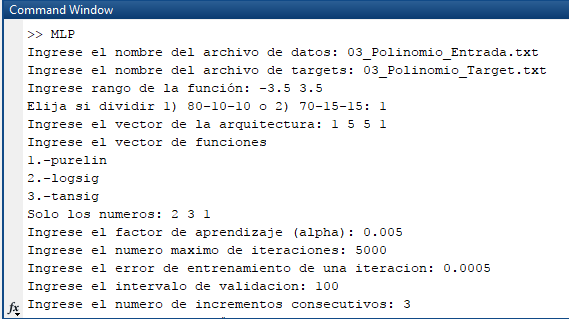
\includegraphics[width=14cm]{3/entrada.png}
        \caption{Entrada de datos del experimento 3.}
        \label{fig:entrada3}
    \end{center}
\end{figure}
En la figura \ref{fig:salida3} se puede observar que la condición de finalización fue que se alcanzo el máximo de iteraciones, por otro lado, el error de aprendizaje fue $5.08 x 10^{-3}$, el error de validación fue $6.606 x 10^{-2}$ y para el error de prueba fue $6.674 x 10^{-2}$.
\begin{figure}[H]
    \begin{center}
        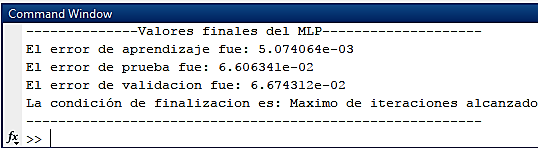
\includegraphics[width=14cm]{3/salida.png}
        \caption{Errores de cada iteración del experimento 3.}
        \label{fig:salida3}
    \end{center}
\end{figure}
Las siguientes imágenes son la evolución de pesos y bias de cada capa. Cada gráfica tiene comportamientos diferentes pero algo en lo que se parecen es que en algún punto de la gráfica ya no se producen tantas modificaciones en los valores que presentan.
\begin{figure}[H]
    \begin{center}
        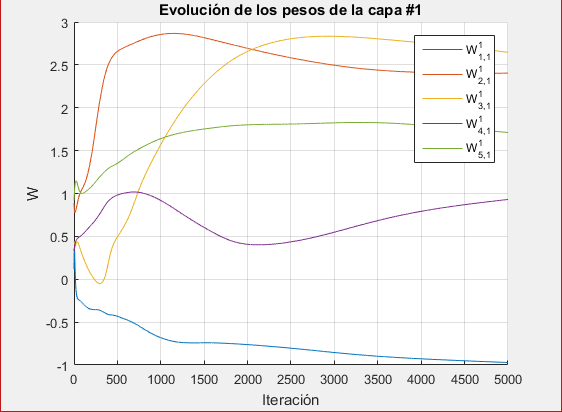
\includegraphics[width=12cm]{3/pesos1.png}
        \caption{Evolución de los pesos de la capa 1 del experimento 3.}
        \label{fig:pesos5}
    \end{center}
\end{figure}

\begin{figure}[H]
    \begin{center}
        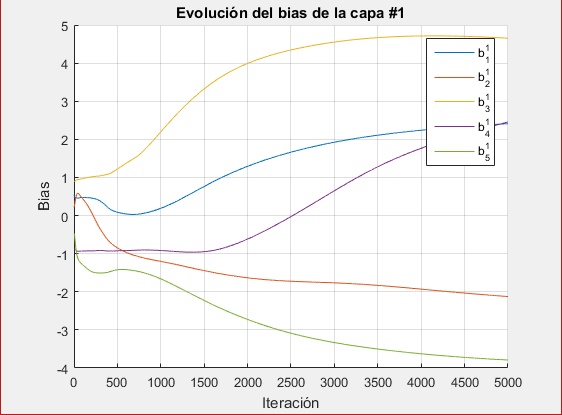
\includegraphics[width=12cm]{3/bias1.png}
        \caption{Evolución de los bias de la capa 1 del experimento 3.}
        \label{fig:bias5}
    \end{center}
\end{figure}

\begin{figure}[H]
    \begin{center}
        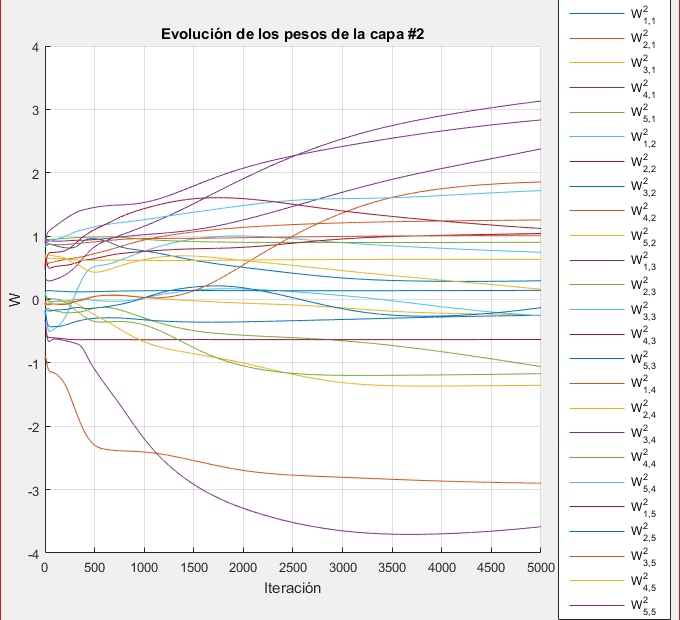
\includegraphics[width=16cm]{3/pesos2.png}
        \caption{Evolución de los pesos de la capa 2.}
        \label{fig:pesos6}
    \end{center}
\end{figure}

\begin{figure}[H]
    \begin{center}
        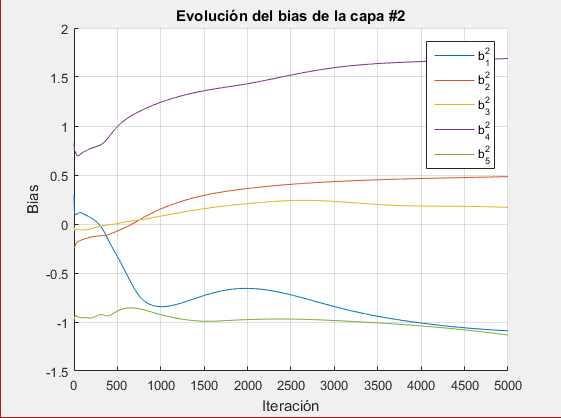
\includegraphics[width=12cm]{3/bias2.png}
        \caption{Evolución de los bias de la capa 2.}
        \label{fig:bias6}
    \end{center}
\end{figure}

\begin{figure}[H]
    \begin{center}
        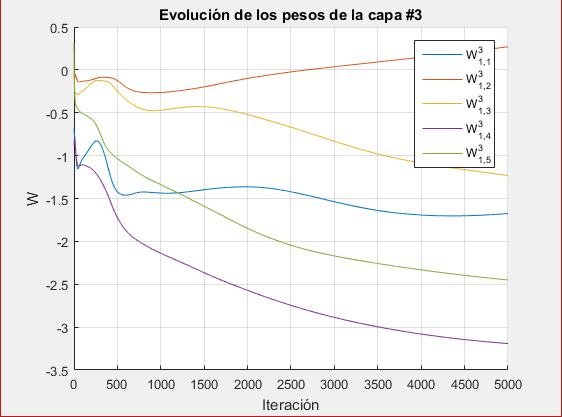
\includegraphics[width=12cm]{3/pesos3.png}
        \caption{Evolución de los pesos de la capa 3.}
        \label{fig:pesos7}
    \end{center}
\end{figure}

\begin{figure}[H]
    \begin{center}
        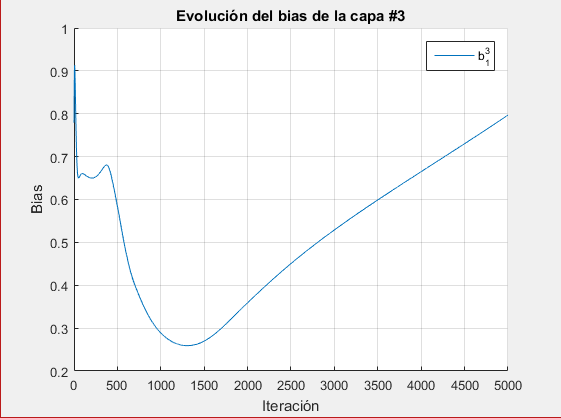
\includegraphics[width=12cm]{3/bias3.png}
        \caption{Evolución de los bias de la capa 3.}
        \label{fig:bias7}
    \end{center}
\end{figure}

Finalmente tenemos la comparación de la salida del MLP y los valores reales, ya que el error es muy bajo la aproximación se realiza en casi todos los puntos con gran precisión a excepción de los extremos de la función en los que hay cambios muy drásticos que no se modelan correctamente.
\begin{figure}[H]
    \begin{center}
        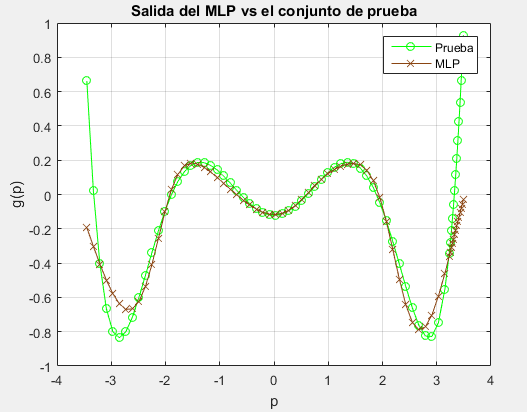
\includegraphics[width=12cm]{3/prueba.png}
        \caption{Comparación de las gráficas}
        \label{fig:prueba3}
    \end{center}
\end{figure}
El comportamiento de la función se puede ver reflejado en la evolución del error en el cual incluso el error de validación es más pequeño con cada iteración que se genera.
\begin{figure}[H]
    \begin{center}
        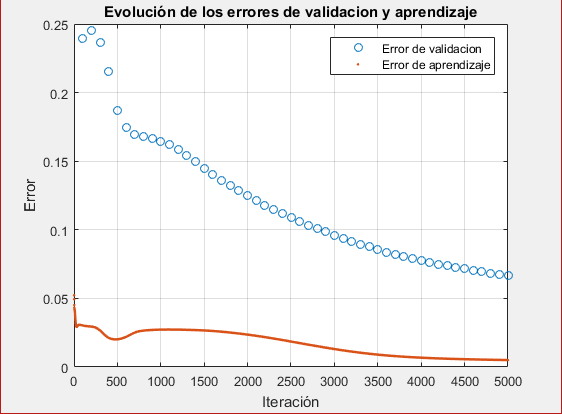
\includegraphics[width=14cm]{3/error.png}
        \caption{Evolución de los dos errores.}
        \label{fig:error3}
    \end{center}
\end{figure}
